\chapter{Technical Background}
\label{sec:state}

% Hier werden zwei wesentliche Aufgaben erledigt:

% 1. Der Leser muß alles beigebracht bekommen, was er zum Verständnis
% der späteren Kapitel braucht. Insbesondere sind in unserem Fach die
% Systemvoraussetzungen zu klären, die man später benutzt. Zulässig ist
% auch, daß man hier auf Tutorials oder Ähnliches verweist, die hier auf
% dem Netz zugänglich sind.

% 2. Es muß klar werden, was anderswo zu diesem Problem gearbeitet
% wird. Insbesondere sollen natürlich die Lücken der anderen klar
% werden. Warum ist die eigene Arbeit, der eigene Ansatz wichtig, um
% hier den Stand der Technik weiterzubringen? Dieses Kapitel wird von
% vielen Lesern übergangen (nicht aber vom Gutachter ;-), auch später
% bei Veröffentlichungen ist "Related Work" eine wichtige Sache.

% Viele Leser stellen dann später fest, daß sie einige der Grundlagen
% doch brauchen und blättern zurück. Deshalb ist es gut,
% Rückwärtsverweise in späteren Kapiteln zu haben, und zwar so, daß man
% die Abschnitte, auf die verwiesen wird, auch für sich lesen
% kann. Diese Kapitel kann relativ lang werden, je größer der Kontext
% der Arbeit, desto länger. Es lohnt sich auch! Den Text kann man unter
% Umständen wiederverwenden, indem man ihn als "Tutorial" zu einem
% Gebiet auch dem Netz zugänglich macht.

% Dadurch gewinnt man manchmal wertvolle Hinweise von Kollegen. Dieses
% Kapitel wird in der Regel zuerst geschrieben und ist das Einfachste
% (oder das Schwerste weil erste).

%\ldots state of the art \ldots

%\todo{write state}
This chapter provides background knowledge of all the content and topics covered in the thesis. This thesis presumes that the reader is 
already aware of the basic concepts of operating system, kubernetes\cite*{k8s}, and confidential computing. Nevertheless, it offers a brief overview of some essential terms and 
concepts to help the reader better understand the later chapters. For a short rundown of associate terminology, please check the glossary on 
this page.
\todo{add glossary page nummber}
\section{Kubernetes}
\begin{figure}[H]
    \centering
    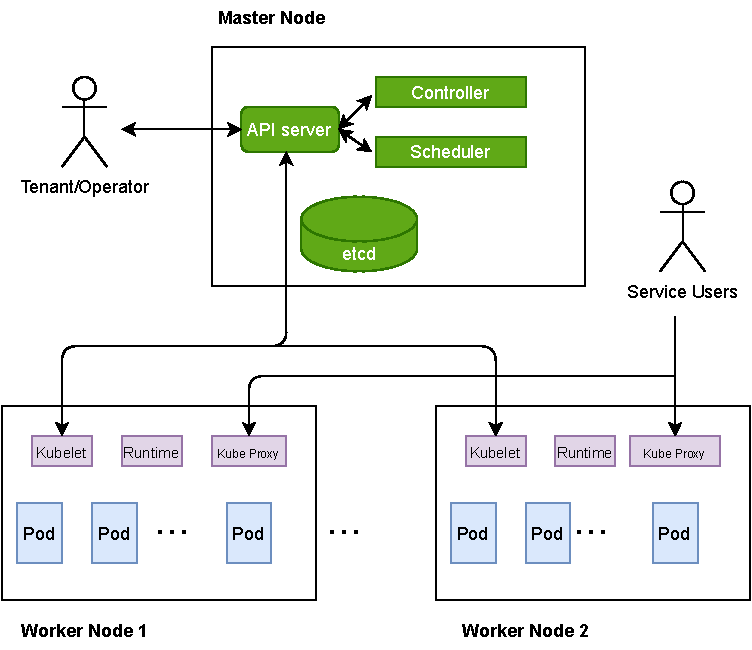
\includegraphics[width=0.8\textwidth]{images/k8s_arch.pdf}
    \caption[k8s arch]{k8s arch}
    \label{fig:k8s_arch}
  \end{figure}
\todo{add description for k8s architectural diagram}

Kubernetes\cite*{k8s} is a portable, scalable open-source platform for managing and orchestrating containerized workloads. Kubernetes emerged because, in the context of the rise of cloud computing, more and more applications are being deployed to the cloud, 
and cloud operators need an automated tool to manage thousands of containers. Kubernetes provides operators with a framework for running cloud-native applications\cite*{KRATZKE20171} in both elastically and resiliently manner. 
It undertakes application scaling and failover and offers a variety of deployment models.

Kubernetes also introduces the concept of pod. In a cluster, a pod, which consists of one or more containers sharing network and storage resources, is the smallest deployment unit managed by Kubernetes. It has a unique cluster-IP address, and the containers within it 
can communicate with each other through the localhost. In addition, Kubernetes support different isolation levels of pods. With the runtime class keyword, clients can choose to deploy pods based on Linux namespace and cgroup for better performance, 
or hardware virtualization for better security\cite*{k8s_runtime_class}.


\subsection{Kubernetes architecture}
From an architectural point of view, a k8s cluster consists of at least one master node and several worker nodes. A node can be a physical or virtual machine. The master node consists of a series of control plane components that make global decisions 
about the cluster, including scheduling, detecting, and responding to cluster events, for example, dynamically adjusting the number of 
pods in an application based on resource utilization. As shown in figure~\ref{fig:k8s_arch}, these control plane components include the apiserver, controller, scheduler, and ectd\cite*{k8s}. Apiserver provides the kubernetes control plane with an 
interface to control and manage the cluster. Specifically, it can be used to receive and authenticate requests from users and other components of the cluster, and update the corresponding API objects that include services pods, and replication 
controllers. Controller is a control loop that continuously monitors the state of the cluster and attempts to move the current state of the cluster to the desired state. For example, the Node controller is responsible for monitoring the state 
of each node and responding accordingly when a node crash. Scheduler continuously search undeployed pods and deploys them to an appropriate worker node. Factors that influence scheduling decisions are resource requirements, 
hardware/software/policy constraints, affinity, data locality, and inter-workload interference. The etcd is a distributed, highly available key-value store for storing cluster level data.

Each worker node, which is managed by the master node runs and maintains the pods. It consists of three main components, kubelet, container runtime (like containerd\cite*{containerd} and ciro\cite*{cri-o}), and kube-proxy. Kubelet is responsible for communication between the 
worker node and the master node and for ensuring that the pods runs properly on the worker node. Container runtime is used to create and manage image and  container lifecycle, which includes pulling images from the remote, unpacking images, 
initializing the container's runtime environment (setting up storage, network), and running the container. The kube-proxy running on each node implements part of the Kubernetes service and maintains network rules on each node, which allows 
network access to pods from both within and outside the cluster

\subsection{Open Standards (CRI\cite*{cri-interface}, OCI\cite*{oci-spec}) makes Kubernetes more extensible}

CRI introduces an abstraction layer that empowers kubelet to work with a diverse range of container runtimes without the need to modify cluster components. It defines the requirements of the 
orchestration system regarding the container runtime and decouples the container runtime from the kubelet source code, which dramatically reduces the effort involved in integrating container 
runtimes into k8s\cite*{cri-interface}.

\todo{add long description for cri overview and k8s with oci cri figure}
\begin{figure}[H]
    \centering
    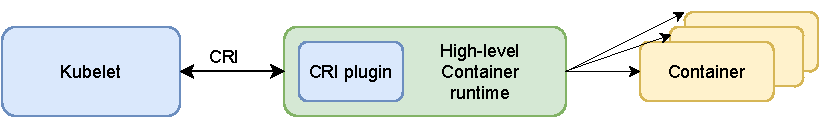
\includegraphics[width=0.8\textwidth]{images/cri_overviwe.pdf}
    \caption[cri overview]{cri overview}
    \label{fig:cri_overviwe}
  \end{figure}


Figure ~\ref{fig:cri_overviwe} shows the overview of CRI. kubelet communicates with the high-level container runtime via sockets, where the high-level container runtime implements a CRI plugin as a socket server according to the CRI 
requirements. The socket server provides two primary services to kubelet, namely ImageService and RuntimeService. The ImageService offers kubelet services such as pulling images from remote and 
inspecting and deleting images managed by the container runtime. The RuntimeService, on the other hand, enables the kubelet to manage the container and sandbox lifecycle 
(RunPodSandbox /StopPodSandbox/RemovePodSandbox/PodSandboxStatus/CreateContainer/StartContainer/StopContainer, etc.) 
and interact with containers (attach/port-forward/exec)\cite*{cri-interface}.

\begin{figure}[H]
    \centering
    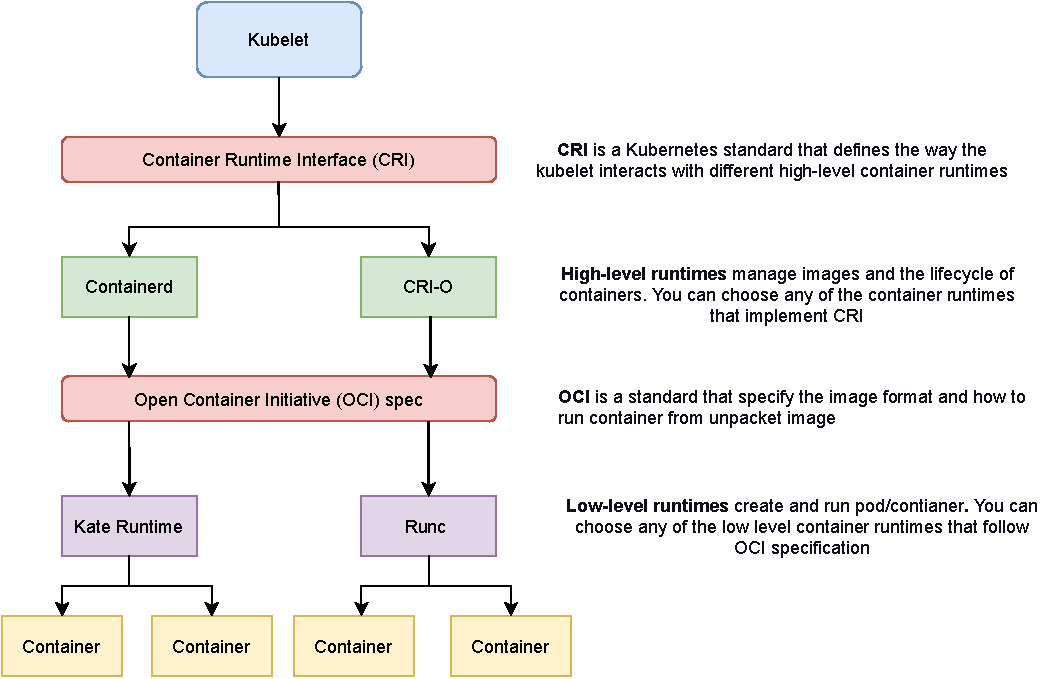
\includegraphics[width=0.8\textwidth]{images/k8s_with_oci_cri.pdf}
    \caption[k8s with oci cri]{k8s with oci cri}
    \label{fig:k8s_with_oci_cri}
\end{figure}
\todo{add long description for  k8s with oci cri figure}
In comparison to CRI, which facilitates easy interaction between kubelet and the various high-level container runtimes that manage the image and container lifecycle, the OCI runtime 
specification\cite*{oci-runtime-spec} defines how low-level container runtimes create and run containers. Typical low-level runtimes are mainly classified as native runtime 
(runc\cite*{runc}, railcar\cite*{railcar}, Crun\cite*{runc}, rkt\cite*{rkt}) , and Sandboxed-virtualized runtimes (kata runtime\cite*{Kata-Containers}, quark runtime\cite*{quark}, gvisor runtime\cite*{gvisor}, etc.). 
We refer the readers to \cite*{Runtime-Comparison} for a comprehensive comparison of these container runtimes. Figure~\ref{fig:k8s_with_oci_cri} summarizes how Kubernetes manages containers through the CRI/OCI interface and a variety of high/low-level container runtimes.

\subsection{Loging}

\section{QUARK CONTAINER}
This section gives a high-level overview of the Quark container\cite*{quark} by introducing its main components and explaining how the guest (Qkenel) communicates with the 
VMM (Qvisor) and host kernel using Hcall ,Qcall, and Ucall, respectively. This explanation is necessary for a better understanding of Chapter 4.

Quark Container is an OCI-compatible container runtime\cite*{oci-runtime-spec}  designed to provide the "security of a virtual machine" while offering the "speed of a 
container\cite*{speed_secure_container_slogen}." It uses KVM hypervisor to launch a virtual machine with a library operating system (Qkernel) written in rust to run containers. 
This container inside VM architecture offers defense in depth. Therefore, a rogue containerized program exploiting a qkernel vulnerability only gains access to qvisor, 
a restricted user process.
Compared to other sandboxed container runtimes, e.g., kata\cite*{Kata-Containers} and gvisor\cite*{gvisor}, using Qkernel as the guest operating system eliminates unnecessary code, 
resulting in a smaller footprint, a faster startup, less overhead, and ensuring the same level of isolation and security for containers\cite*{quark_performance_report}.
\subsection{Architecture}
\begin{figure}[H]
    \centering
    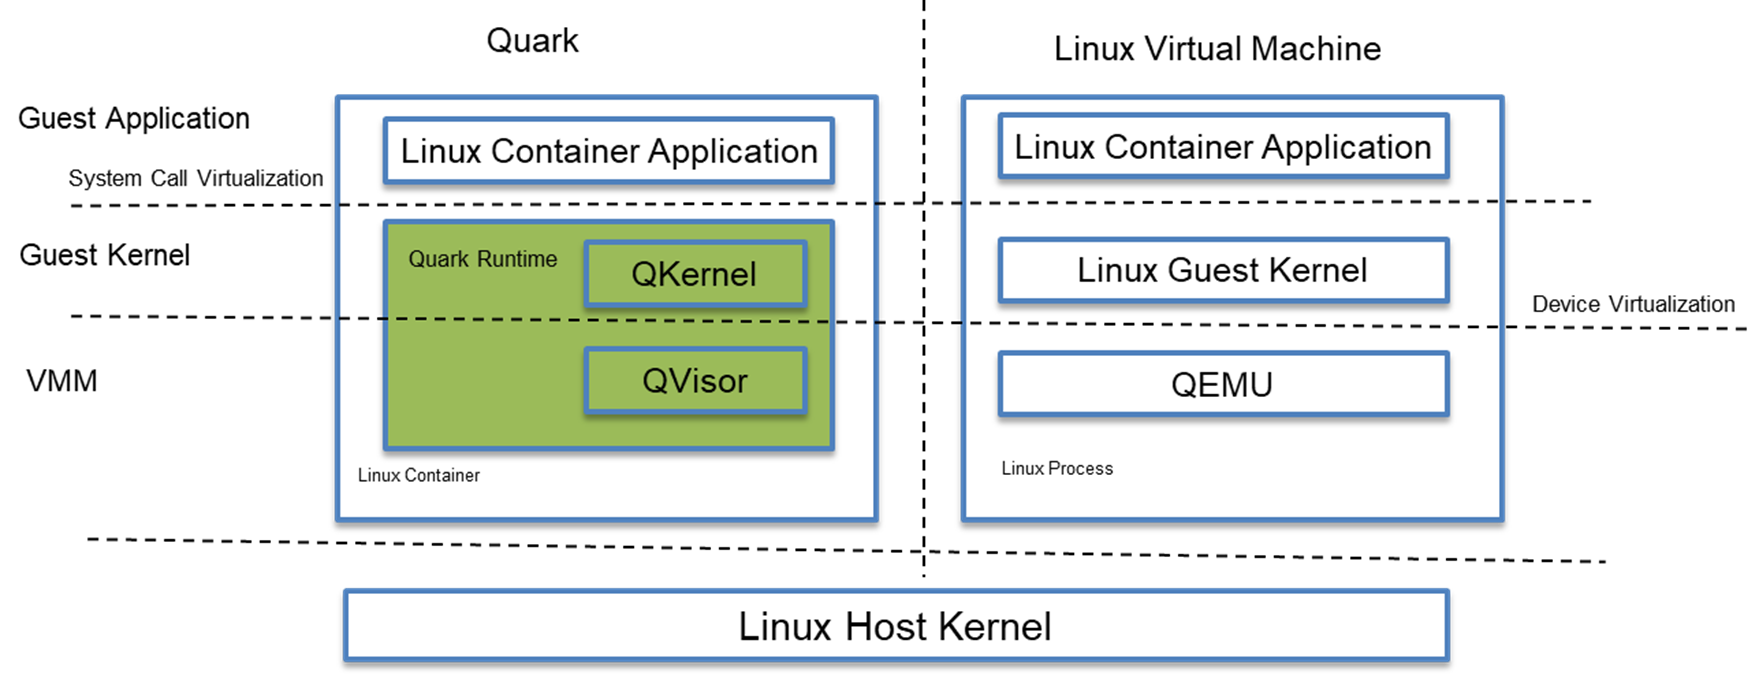
\includegraphics[width=0.8\textwidth]{images/quark_design.png}
    \caption[quark design]{quark design}
    \label{fig:quark_design}
\end{figure}
\todo{add long description for quark design}

In Figure ~\ref{fig:quark_design}, we can see the architecture comparison between Quark-based and Linux virtual machines. The Quark-based virtual machine is shown on the left. This virtual machine consists of Qvisor, 
Qkernel, and several containerized applications. Corresponding to qemu in a Linux virtual machine, qvisor is a virtual machine manager that uses KVM to create and manage the qkernel-based micro VM. 
The qkernel and the containerized applications comprise a virtual machine, where the qkernel serves as the guest operating system and applications run as processes in the guest user space. Unlike 
the Linux guest kernel, qkernel is an ultra-lightweight kernel that contains only necessary code. Furthermore, it implements essential operating system components, such as process management, 
memory management, file system, and network system. Thus, the qkernel, like a macro kernel, provides services to the running program. The user program, in turn, accesses these services via guest 
system calls. i.e., X86-64 SysCall/SysRet. The individual components in the qkernel are implemented with the help of the qvisor and the host kernel. When a user program triggers a guest system call, the qkernel makes use of 
various interfaces to access the services in the qvisor and the host kernel in order to complete the system call. As can be seen in Figure ~\ref{fig:quark_io}, these interfaces include hyper call, qcall, and ucall.

\begin{figure}[H]
    \centering
    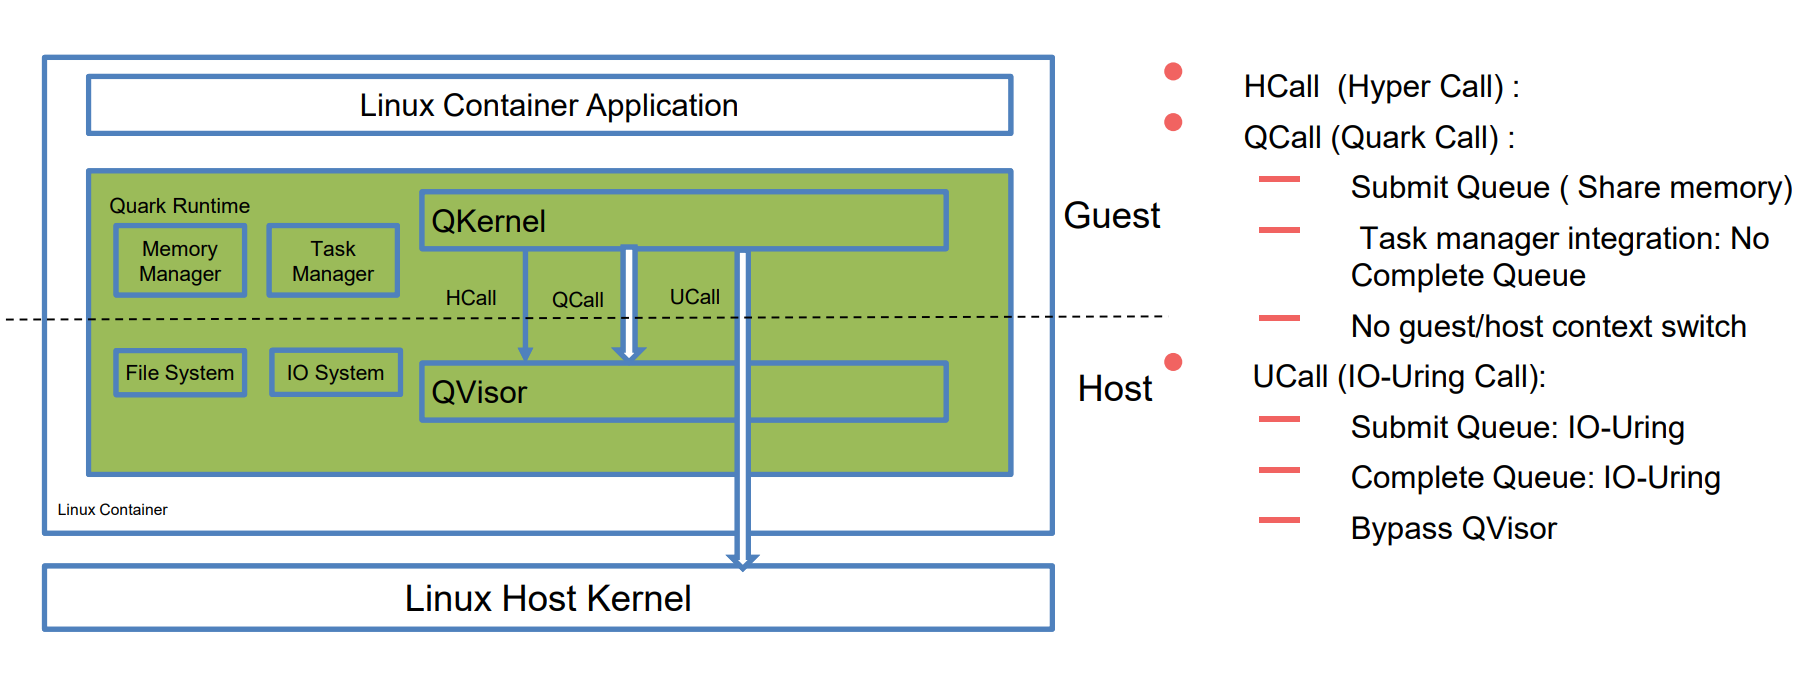
\includegraphics[width=0.8\textwidth]{images/quark_io.png}
    \caption[quark IO]{quark IO}
    \label{fig:quark_io}
\end{figure}

\todo{add long description for quark IO, modify the image: add Guest System Call btw. container app and qkernel}

\subsection{Qcall, Hypercall, and Ucall}
\begin{figure}[H]
  \centering
  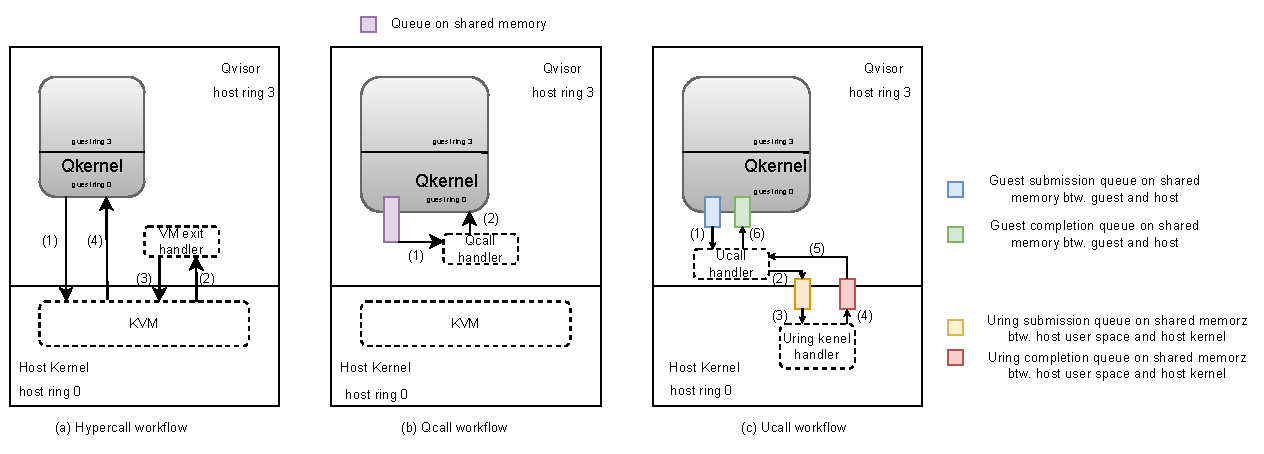
\includegraphics[width=0.8\textwidth]{images/hypercall_qcall_ucall.pdf}
  \caption[Workflow of Hypercall, Qcall, and Ucall]{Workflow of Hypercall, Qcall, and Ucall}
  \label{fig:hypercall_qcall_ucall}
\end{figure}
\todo{describe the workflow of Hypercall, Qcall, and Ucall in figure's long description}
Hypercall provides the qkernel with the means to issue commands to the Qvisor. Figure ~\ref{fig:hypercall_qcall_ucall}(a) shows the hypercall workflow in the context of Quark. 
When qkernel triggers a hypercall, the CPU leaves guest ring 0 mode and enters host ring 0 mode (~\ref{fig:hypercall_qcall_ucall}a (1)). KVM then checks the reason for the VM exit by examining the VMCB and forwards the 
hypercall to Qvisor running on host ring 3 mode (~\ref{fig:hypercall_qcall_ucall}a (2)). After handling the hypercall request, Qvisor invokes KVM, which resumes qkernel execution in guest ring 0 mode (~\ref{fig:hypercall_qcall_ucall}a (3), (4)).
With hypercall, the Qkernel can access service in Qvisor, such as opening a file, initializing IO. Unfortunately, 
this approach is very expensive due to the context switching between the Qkenel and Qvisor. 

To this end, Quark provides an asynchronous mechanism called Qcall as an alternative. 
As shown in Figure ~\ref{fig:hypercall_qcall_ucall}(b), this mechanism is implemented by a queue on shared memory between the Qkernel and the Qvisor and an io thread on the Qvisor side, where the
shared queue is used to transfer requests sent by the Qkernel to the Qvisor, and the io thread is responsible for retrieving requests from the queue and notifying the Qkernel thread when the Qivosr completes 
the request. Through this mechanism, Qkernel is able to access services in Qvisor in an asynchronous manner without VM exit, which improves the performance of the Qkernel significantly.

Typically, IO operations with hypercall are expensive. Therefore, Quark introduced the Ucall interface as a means of direct communication between the Qkernel and the host kernel for host 
IO data operations,  such as socket reading and writing. It supports both synchronous and asynchronous IO operations. Figure ~\ref{fig:hypercall_qcall_ucall}(c) details the workflow of the Qkernel 
using Ucall for synchronous IO operations. First, the qkernel thread submits the IO request into the guest submission queue (Figure ~\ref{fig:hypercall_qcall_ucall}c (1)). Then the Qvisor Ucall handler thread copies the request to the uring submission 
queue (Figure ~\ref{fig:hypercall_qcall_ucall}c (2)). After the Uring kernel hander finishes processing the IO request, it puts the IO processing result into the uring completion queue (Figure ~\ref{fig:hypercall_qcall_ucall}c (3), (4)). The result 
contains a user\_data field, which is submitted from the initial IO request and contains information about the Qkernel thread that submitted the IO request. By reading this field, the Qvisor Ucall handler thread wakes up the corresponding Qkernel thread 
after copying the IO processing result to the guest completion queue (Figure ~\ref{fig:hypercall_qcall_ucall}c (5), (6)).



\section{TEE --generic Idea}
The hardware-assisted Trusted Execution Environment (TEE) provides one or more tamper-proof computing environments that ensure data confidentiality and integrity. Such environment is also called enclave. It protects security-sensitive applications from co-located attackers 
through verifiable boot of the execution environment, CPU and memory isolation, trusted IO, and secure storage\cite*{Hardware-supported-TEE}. This security guarantee relays on specialized chips. Therefore, breaking various software layers,
such as operating systems and hypervisors, do not affect TEE's ability to protect sensitive computation and data\cite*{7345265}.

As shown in Figure ~\ref{fig:vm_process_tee}, hardware-based TEE models can be conceptually divided into two categories, namely VM-based TEE and process-based TEE\cite*{101145}. In VM-based TEE models, the entire VM memory is encrypted with a hardware-based encryption key to protect the VM from other privileged 
software components, such as hypervisor and operating system. Examples of VM-based TEE include AMD SEV\cite*{AMD_SEV}, INTEL TDX\cite*{Inte_TDX}, etc. On the other hand, process-based TEE encrypts only a segment of memory in the application address space,  i.e., the address 
space is divided into two parts, a trusted region and an untrusted region, which communicate with each other through call gates. 
Examples of process-based TEE implementation 
are INTEL SGX\cite*{INTEL_SGX} and OpenPOWER's Sanctum\cite*{Costan2016SanctumMH}.
\begin{figure}[H]
  \centering
  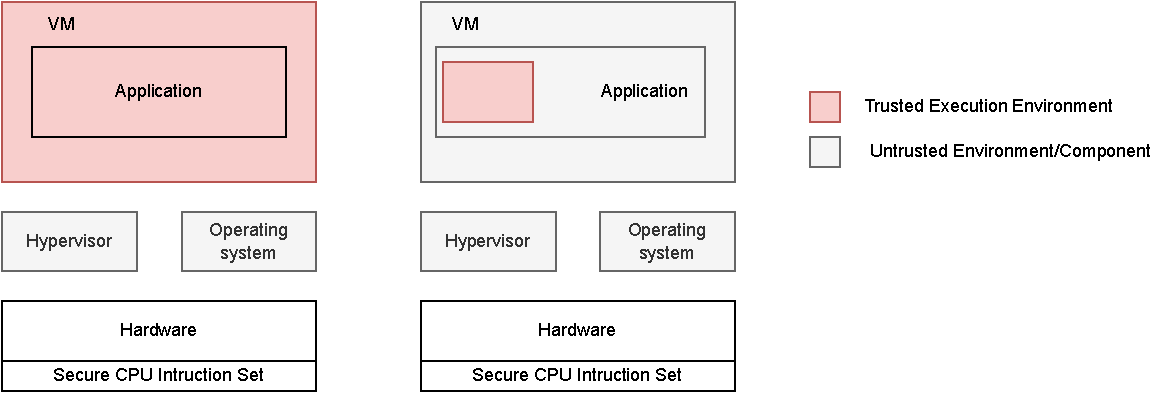
\includegraphics[width=0.8\textwidth]{images/vm_process_tee.pdf}
  \caption[VM based vs process based TEE model]{VM based vs process based TEE model}
  \label{fig:vm_process_tee}
\end{figure}

Both of these models have their advantages and disadvantages\cite*{10.3389/fcomp.2022.930741} \cite*{Execution_Environment_landscape} \cite*{101145}. Take Intel SGX as an example of process-based TEE. Compared to VM-based TEE, it has the advantage of a smaller TCB, i.e., a smaller attack surface. However, the disadvantages are also obvious. A frequently 
cited disadvantage is the need for significant software modifications to accommodate this TEE model. Other drawbacks include performance degradation due to limited EPC size in case a process requires a huge area of encrypted memory. Furthermore, this model 
may cause a significant performance penalty for IO-intensive applications, as it only allows enclave to perform system calls and hardware accesses via Ocall and Ecall, which can be very expensive.


The VM-based approach has the following advantages. First, the model provides bi-directional isolation, alleviating the concern about malware running in the enclave corrupting the other components on the same host. In addition, the model is more 
flexible compared to process base approaches as it supports running security-sensitive programs in an enclave (VM) without modification. However, placing the entire virtual machine under the protection of the TEE increases the TCB, making the approach more vulnerable to attacks.


In the next two sections, we describe in more detail how VM-based TEE safeguards sensitive data by means of memory encryption, attestation, etc. We choose AMD SEV and INTEL TDX as examples and compare their differences since they may be widely used by the industry in the future.
Also, since our implementation is based on VM-based TEE, 
a detailed description of process-based TEE is considered out of the scope. For a detailed explanation of process-based TEE, we refer the reader to \cite*{cryptoeprint:2016/086} \cite*{10.1145/2487726.2488370} \cite*{SGX_PAPER_LIST}.


\subsection{AMD SEV SNP}
AMD SEV SNP is AMD's latest virtual machine-based TEE solution. It retains the features of its predecessor, namely VM memory encryption, register state protection after VM exit, and further adds integrity protection for encrypted memory.

AMD SEV SNP protects the virtual machine's memory with encryption. When a service running in an enclave (VM) accesses memory, the AES-128 encryption engine embedded in the memory controller transparently encrypts or decrypts the memory using a memory encryption key. Note that each enclave is assigned a unique memory encryption, and this key will never be revealed to an untrusted entity, such as a hypervisor. As a result, untrusted entities can only read the cipher text on the VM's memory. To enable sharing of memory pages between enclaves or between an enclave and hypervisor, a new control bit, the "C-bit," is introduced in the page table entry, allowing the enclave to decide which page should be encrypted.

To mitigate attacks on VM control blocks during VM exits, SNP supports non-automatic VM exits. SNP classifies VM exits into two categories: automatic VM exits and non-automatic VM exits. Automatic VM exits refer to VM exits that do not expose any guest register state to the hypervisor. Examples of automatic VM exits include those triggered by physical interrupts, shutdowns, and the hlt instruction, etc. All other exits are non-automatic VM exits, i.e., exits of VMs that require exposing the state of the guest registers to the hypervisor. In this case, SNP allows the guest to select the registers that need to be exposed to the hypervisor and encrypt the remaining register state before the VM exits.

In comparison to its predecessor, AMD SNP protects the integrity of enclave memory by introducing RMP, which helps SNP enforce the ownership of a physical page to one entity, i.e., only the owner of a page can modify that page. In addition, changing the ownership of a page will erase the contents of that page. In this way, malicious entities may only read the encrypted virtual machine memory rather than modify it.

SEV SNP also supports attestation. It allows the secret owner to verify the trustworthiness of the enclave and decide whether to make the secrets in their possession available to the enclave. 
This process is also referred to as attestation and provisioning. Compared to its predecessors, AMD SEV, and AMD SEV-ES, SNP not only retains the static attestation, i.e., the attestation during 
enclave launch, but also adds the runtime attestation feature. This feature makes the SNP's attestation more flexible as it allows the verifier to examine the trustworthiness of the enclave at 
any time while it is running. It is also interesting to note that the AMD SEV family does not support local attestation compared to intel's TEE solutions. As such, this section skips the 
explanation of local attestation. For those interested in local attestation, please refer to the next section on Intel TDX.

Remote attestation for SEV SNP relies on three keys, the  Chip Endorsement Key (CEK), the e AMD SEV Signing Key (ASK), and the AMD root signing key(RSK), to establish 
the root of trust. CEK is a P-384 ECDSA chip-unique signing key fused into the processor die, while ASK and ARK are global keys securely stored by AMD. The relationship between these three keys is 
that CEK on each AMD platform is signed by ASK, and ASK is signed by ARK. During the operation of the enclave, the certifier can request an attestation report signed by the CEK from the enclave. 
This report contains measurements related to the enclave, which include measurements on the contents of the enclave memory, the configuration of the platform on which the enclave is running, etc.
 In addition, the report includes a 512-bit custom guest data field to, for example, prove freshness to the verifier or establish a mutual TLS communication channel between the enclave and the 
 verifier. In the end, after obtaining the report, the verifier can verify the report using the public key of the AMD signature key obtained from AMD and decide whether the enclave should be 
 provisioned based on the measurements in the report.

\subsection{Intel TDX}
\subsection{Comparison}

\section{ACCESS CONTROL}


\section{Summary}
In this chapter, I first give an overview of the various components of k8s and two standards that make k8s more extensible. Furthermore, I depict the general architecture of the quark container 
and the interfaces that qkernel used to communicate with qvisor and host kernel. Last but not least, I describe the concepts related to TEE, such as memory protection, attestation.

\cleardoublepage

%%% Local Variables:
%%% TeX-master: "diplom"
%%% End:
